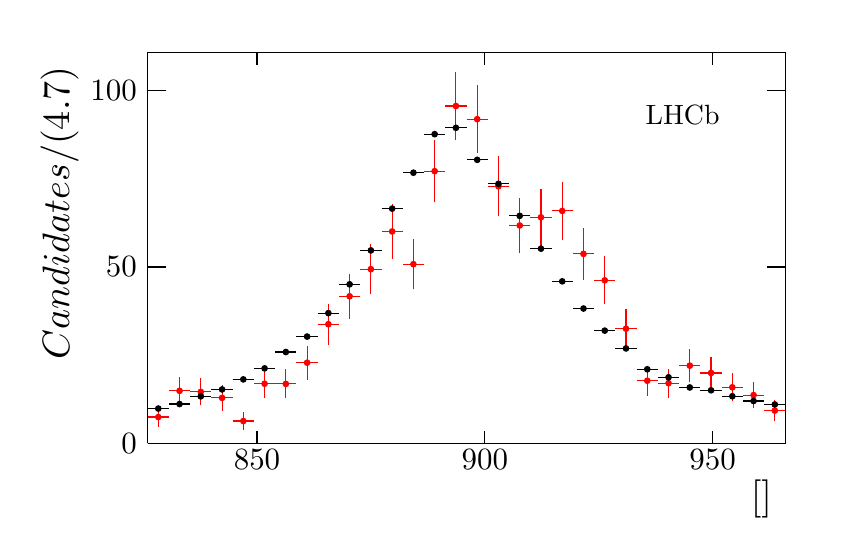
\begin{tikzpicture}
\pgfdeclareplotmark{cross} {
\pgfpathmoveto{\pgfpoint{-0.3\pgfplotmarksize}{\pgfplotmarksize}}
\pgfpathlineto{\pgfpoint{+0.3\pgfplotmarksize}{\pgfplotmarksize}}
\pgfpathlineto{\pgfpoint{+0.3\pgfplotmarksize}{0.3\pgfplotmarksize}}
\pgfpathlineto{\pgfpoint{+1\pgfplotmarksize}{0.3\pgfplotmarksize}}
\pgfpathlineto{\pgfpoint{+1\pgfplotmarksize}{-0.3\pgfplotmarksize}}
\pgfpathlineto{\pgfpoint{+0.3\pgfplotmarksize}{-0.3\pgfplotmarksize}}
\pgfpathlineto{\pgfpoint{+0.3\pgfplotmarksize}{-1.\pgfplotmarksize}}
\pgfpathlineto{\pgfpoint{-0.3\pgfplotmarksize}{-1.\pgfplotmarksize}}
\pgfpathlineto{\pgfpoint{-0.3\pgfplotmarksize}{-0.3\pgfplotmarksize}}
\pgfpathlineto{\pgfpoint{-1.\pgfplotmarksize}{-0.3\pgfplotmarksize}}
\pgfpathlineto{\pgfpoint{-1.\pgfplotmarksize}{0.3\pgfplotmarksize}}
\pgfpathlineto{\pgfpoint{-0.3\pgfplotmarksize}{0.3\pgfplotmarksize}}
\pgfpathclose
\pgfusepathqstroke
}
\pgfdeclareplotmark{cross*} {
\pgfpathmoveto{\pgfpoint{-0.3\pgfplotmarksize}{\pgfplotmarksize}}
\pgfpathlineto{\pgfpoint{+0.3\pgfplotmarksize}{\pgfplotmarksize}}
\pgfpathlineto{\pgfpoint{+0.3\pgfplotmarksize}{0.3\pgfplotmarksize}}
\pgfpathlineto{\pgfpoint{+1\pgfplotmarksize}{0.3\pgfplotmarksize}}
\pgfpathlineto{\pgfpoint{+1\pgfplotmarksize}{-0.3\pgfplotmarksize}}
\pgfpathlineto{\pgfpoint{+0.3\pgfplotmarksize}{-0.3\pgfplotmarksize}}
\pgfpathlineto{\pgfpoint{+0.3\pgfplotmarksize}{-1.\pgfplotmarksize}}
\pgfpathlineto{\pgfpoint{-0.3\pgfplotmarksize}{-1.\pgfplotmarksize}}
\pgfpathlineto{\pgfpoint{-0.3\pgfplotmarksize}{-0.3\pgfplotmarksize}}
\pgfpathlineto{\pgfpoint{-1.\pgfplotmarksize}{-0.3\pgfplotmarksize}}
\pgfpathlineto{\pgfpoint{-1.\pgfplotmarksize}{0.3\pgfplotmarksize}}
\pgfpathlineto{\pgfpoint{-0.3\pgfplotmarksize}{0.3\pgfplotmarksize}}
\pgfpathclose
\pgfusepathqfillstroke
}
\pgfdeclareplotmark{newstar} {
\pgfpathmoveto{\pgfqpoint{0pt}{\pgfplotmarksize}}
\pgfpathlineto{\pgfqpointpolar{44}{0.5\pgfplotmarksize}}
\pgfpathlineto{\pgfqpointpolar{18}{\pgfplotmarksize}}
\pgfpathlineto{\pgfqpointpolar{-20}{0.5\pgfplotmarksize}}
\pgfpathlineto{\pgfqpointpolar{-54}{\pgfplotmarksize}}
\pgfpathlineto{\pgfqpointpolar{-90}{0.5\pgfplotmarksize}}
\pgfpathlineto{\pgfqpointpolar{234}{\pgfplotmarksize}}
\pgfpathlineto{\pgfqpointpolar{198}{0.5\pgfplotmarksize}}
\pgfpathlineto{\pgfqpointpolar{162}{\pgfplotmarksize}}
\pgfpathlineto{\pgfqpointpolar{134}{0.5\pgfplotmarksize}}
\pgfpathclose
\pgfusepathqstroke
}
\pgfdeclareplotmark{newstar*} {
\pgfpathmoveto{\pgfqpoint{0pt}{\pgfplotmarksize}}
\pgfpathlineto{\pgfqpointpolar{44}{0.5\pgfplotmarksize}}
\pgfpathlineto{\pgfqpointpolar{18}{\pgfplotmarksize}}
\pgfpathlineto{\pgfqpointpolar{-20}{0.5\pgfplotmarksize}}
\pgfpathlineto{\pgfqpointpolar{-54}{\pgfplotmarksize}}
\pgfpathlineto{\pgfqpointpolar{-90}{0.5\pgfplotmarksize}}
\pgfpathlineto{\pgfqpointpolar{234}{\pgfplotmarksize}}
\pgfpathlineto{\pgfqpointpolar{198}{0.5\pgfplotmarksize}}
\pgfpathlineto{\pgfqpointpolar{162}{\pgfplotmarksize}}
\pgfpathlineto{\pgfqpointpolar{134}{0.5\pgfplotmarksize}}
\pgfpathclose
\pgfusepathqfillstroke
}
\definecolor{c}{rgb}{1,1,1};
\draw [color=c, fill=c] (0,0) rectangle (10,6.27517);
\draw [color=c, fill=c] (1.4,1.00403) rectangle (9.5,5.96141);
\definecolor{c}{rgb}{0,0,0};
\draw [c] (1.4,1.00403) -- (1.4,5.96141) -- (9.5,5.96141) -- (9.5,1.00403) -- (1.4,1.00403);
\definecolor{c}{rgb}{1,1,1};
\draw [color=c, fill=c] (1.4,1.00403) rectangle (9.5,5.96141);
\definecolor{c}{rgb}{0,0,0};
\draw [c] (1.4,1.00403) -- (1.4,5.96141) -- (9.5,5.96141) -- (9.5,1.00403) -- (1.4,1.00403);
\definecolor{c}{rgb}{1,0,0};
\draw [c,line width=0.4] (1.535,1.21521) -- (1.535,1.33737);
\draw [c,line width=0.4] (1.535,1.33737) -- (1.535,1.45953);
\draw [c,line width=0.4] (1.4,1.33737) -- (1.535,1.33737);
\draw [c,line width=0.4] (1.535,1.33737) -- (1.67,1.33737);
\foreach \P in {(1.535,1.33737)}{\draw[mark options={color=c,fill=c},mark size=2.402402pt,mark=*,mark size=1pt] plot coordinates {\P};}
\draw [c,line width=0.4] (1.805,1.49722) -- (1.805,1.66987);
\draw [c,line width=0.4] (1.805,1.66987) -- (1.805,1.84252);
\draw [c,line width=0.4] (1.67,1.66987) -- (1.805,1.66987);
\draw [c,line width=0.4] (1.805,1.66987) -- (1.94,1.66987);
\foreach \P in {(1.805,1.66987)}{\draw[mark options={color=c,fill=c},mark size=2.402402pt,mark=*,mark size=1pt] plot coordinates {\P};}
\draw [c,line width=0.4] (2.075,1.48566) -- (2.075,1.65658);
\draw [c,line width=0.4] (2.075,1.65658) -- (2.075,1.82749);
\draw [c,line width=0.4] (1.94,1.65658) -- (2.075,1.65658);
\draw [c,line width=0.4] (2.075,1.65658) -- (2.21,1.65658);
\foreach \P in {(2.075,1.65658)}{\draw[mark options={color=c,fill=c},mark size=2.402402pt,mark=*,mark size=1pt] plot coordinates {\P};}
\draw [c,line width=0.4] (2.345,1.41972) -- (2.345,1.58035);
\draw [c,line width=0.4] (2.345,1.58035) -- (2.345,1.74097);
\draw [c,line width=0.4] (2.21,1.58035) -- (2.345,1.58035);
\draw [c,line width=0.4] (2.345,1.58035) -- (2.48,1.58035);
\foreach \P in {(2.345,1.58035)}{\draw[mark options={color=c,fill=c},mark size=2.402402pt,mark=*,mark size=1pt] plot coordinates {\P};}
\draw [c,line width=0.4] (2.615,1.17396) -- (2.615,1.2864);
\draw [c,line width=0.4] (2.615,1.2864) -- (2.615,1.39883);
\draw [c,line width=0.4] (2.48,1.2864) -- (2.615,1.2864);
\draw [c,line width=0.4] (2.615,1.2864) -- (2.75,1.2864);
\foreach \P in {(2.615,1.2864)}{\draw[mark options={color=c,fill=c},mark size=2.402402pt,mark=*,mark size=1pt] plot coordinates {\P};}
\draw [c,line width=0.4] (2.885,1.57625) -- (2.885,1.76025);
\draw [c,line width=0.4] (2.885,1.76025) -- (2.885,1.94424);
\draw [c,line width=0.4] (2.75,1.76025) -- (2.885,1.76025);
\draw [c,line width=0.4] (2.885,1.76025) -- (3.02,1.76025);
\foreach \P in {(2.885,1.76025)}{\draw[mark options={color=c,fill=c},mark size=2.402402pt,mark=*,mark size=1pt] plot coordinates {\P};}
\draw [c,line width=0.4] (3.155,1.57448) -- (3.155,1.75823);
\draw [c,line width=0.4] (3.155,1.75823) -- (3.155,1.94198);
\draw [c,line width=0.4] (3.02,1.75823) -- (3.155,1.75823);
\draw [c,line width=0.4] (3.155,1.75823) -- (3.29,1.75823);
\foreach \P in {(3.155,1.75823)}{\draw[mark options={color=c,fill=c},mark size=2.402402pt,mark=*,mark size=1pt] plot coordinates {\P};}
\draw [c,line width=0.4] (3.425,1.81321) -- (3.425,2.02724);
\draw [c,line width=0.4] (3.425,2.02724) -- (3.425,2.24126);
\draw [c,line width=0.4] (3.29,2.02724) -- (3.425,2.02724);
\draw [c,line width=0.4] (3.425,2.02724) -- (3.56,2.02724);
\foreach \P in {(3.425,2.02724)}{\draw[mark options={color=c,fill=c},mark size=2.402402pt,mark=*,mark size=1pt] plot coordinates {\P};}
\draw [c,line width=0.4] (3.695,2.25571) -- (3.695,2.51587);
\draw [c,line width=0.4] (3.695,2.51587) -- (3.695,2.77603);
\draw [c,line width=0.4] (3.56,2.51587) -- (3.695,2.51587);
\draw [c,line width=0.4] (3.695,2.51587) -- (3.83,2.51587);
\foreach \P in {(3.695,2.51587)}{\draw[mark options={color=c,fill=c},mark size=2.402402pt,mark=*,mark size=1pt] plot coordinates {\P};}
\draw [c,line width=0.4] (3.965,2.58184) -- (3.965,2.87094);
\draw [c,line width=0.4] (3.965,2.87094) -- (3.965,3.16004);
\draw [c,line width=0.4] (3.83,2.87094) -- (3.965,2.87094);
\draw [c,line width=0.4] (3.965,2.87094) -- (4.1,2.87094);
\foreach \P in {(3.965,2.87094)}{\draw[mark options={color=c,fill=c},mark size=2.402402pt,mark=*,mark size=1pt] plot coordinates {\P};}
\draw [c,line width=0.4] (4.235,2.90073) -- (4.235,3.21536);
\draw [c,line width=0.4] (4.235,3.21536) -- (4.235,3.53);
\draw [c,line width=0.4] (4.1,3.21536) -- (4.235,3.21536);
\draw [c,line width=0.4] (4.235,3.21536) -- (4.37,3.21536);
\foreach \P in {(4.235,3.21536)}{\draw[mark options={color=c,fill=c},mark size=2.402402pt,mark=*,mark size=1pt] plot coordinates {\P};}
\draw [c,line width=0.4] (4.505,3.34704) -- (4.505,3.69406);
\draw [c,line width=0.4] (4.505,3.69406) -- (4.505,4.04109);
\draw [c,line width=0.4] (4.37,3.69406) -- (4.505,3.69406);
\draw [c,line width=0.4] (4.505,3.69406) -- (4.64,3.69406);
\foreach \P in {(4.505,3.69406)}{\draw[mark options={color=c,fill=c},mark size=2.402402pt,mark=*,mark size=1pt] plot coordinates {\P};}
\draw [c,line width=0.4] (4.775,2.95942) -- (4.775,3.27852);
\draw [c,line width=0.4] (4.775,3.27852) -- (4.775,3.59762);
\draw [c,line width=0.4] (4.64,3.27852) -- (4.775,3.27852);
\draw [c,line width=0.4] (4.775,3.27852) -- (4.91,3.27852);
\foreach \P in {(4.775,3.27852)}{\draw[mark options={color=c,fill=c},mark size=2.402402pt,mark=*,mark size=1pt] plot coordinates {\P};}
\draw [c,line width=0.4] (5.045,4.06677) -- (5.045,4.46011);
\draw [c,line width=0.4] (5.045,4.46011) -- (5.045,4.85346);
\draw [c,line width=0.4] (4.91,4.46011) -- (5.045,4.46011);
\draw [c,line width=0.4] (5.045,4.46011) -- (5.18,4.46011);
\foreach \P in {(5.045,4.46011)}{\draw[mark options={color=c,fill=c},mark size=2.402402pt,mark=*,mark size=1pt] plot coordinates {\P};}
\draw [c,line width=0.4] (5.315,4.84954) -- (5.315,5.28744);
\draw [c,line width=0.4] (5.315,5.28744) -- (5.315,5.72534);
\draw [c,line width=0.4] (5.18,5.28744) -- (5.315,5.28744);
\draw [c,line width=0.4] (5.315,5.28744) -- (5.45,5.28744);
\foreach \P in {(5.315,5.28744)}{\draw[mark options={color=c,fill=c},mark size=2.402402pt,mark=*,mark size=1pt] plot coordinates {\P};}
\draw [c,line width=0.4] (5.585,4.6908) -- (5.585,5.12006);
\draw [c,line width=0.4] (5.585,5.12006) -- (5.585,5.54932);
\draw [c,line width=0.4] (5.45,5.12006) -- (5.585,5.12006);
\draw [c,line width=0.4] (5.585,5.12006) -- (5.72,5.12006);
\foreach \P in {(5.585,5.12006)}{\draw[mark options={color=c,fill=c},mark size=2.402402pt,mark=*,mark size=1pt] plot coordinates {\P};}
\draw [c,line width=0.4] (5.855,3.88595) -- (5.855,4.26822);
\draw [c,line width=0.4] (5.855,4.26822) -- (5.855,4.65049);
\draw [c,line width=0.4] (5.72,4.26822) -- (5.855,4.26822);
\draw [c,line width=0.4] (5.855,4.26822) -- (5.99,4.26822);
\foreach \P in {(5.855,4.26822)}{\draw[mark options={color=c,fill=c},mark size=2.402402pt,mark=*,mark size=1pt] plot coordinates {\P};}
\draw [c,line width=0.4] (6.125,3.41805) -- (6.125,3.76993);
\draw [c,line width=0.4] (6.125,3.76993) -- (6.125,4.12182);
\draw [c,line width=0.4] (5.99,3.76993) -- (6.125,3.76993);
\draw [c,line width=0.4] (6.125,3.76993) -- (6.26,3.76993);
\foreach \P in {(6.125,3.76993)}{\draw[mark options={color=c,fill=c},mark size=2.402402pt,mark=*,mark size=1pt] plot coordinates {\P};}
\draw [c,line width=0.4] (6.395,3.51549) -- (6.395,3.87393);
\draw [c,line width=0.4] (6.395,3.87393) -- (6.395,4.23237);
\draw [c,line width=0.4] (6.26,3.87393) -- (6.395,3.87393);
\draw [c,line width=0.4] (6.395,3.87393) -- (6.53,3.87393);
\foreach \P in {(6.395,3.87393)}{\draw[mark options={color=c,fill=c},mark size=2.402402pt,mark=*,mark size=1pt] plot coordinates {\P};}
\draw [c,line width=0.4] (6.665,3.5914) -- (6.665,3.95486);
\draw [c,line width=0.4] (6.665,3.95486) -- (6.665,4.31832);
\draw [c,line width=0.4] (6.53,3.95486) -- (6.665,3.95486);
\draw [c,line width=0.4] (6.665,3.95486) -- (6.8,3.95486);
\foreach \P in {(6.665,3.95486)}{\draw[mark options={color=c,fill=c},mark size=2.402402pt,mark=*,mark size=1pt] plot coordinates {\P};}
\draw [c,line width=0.4] (6.935,3.08114) -- (6.935,3.40928);
\draw [c,line width=0.4] (6.935,3.40928) -- (6.935,3.73743);
\draw [c,line width=0.4] (6.8,3.40928) -- (6.935,3.40928);
\draw [c,line width=0.4] (6.935,3.40928) -- (7.07,3.40928);
\foreach \P in {(6.935,3.40928)}{\draw[mark options={color=c,fill=c},mark size=2.402402pt,mark=*,mark size=1pt] plot coordinates {\P};}
\draw [c,line width=0.4] (7.205,2.76932) -- (7.205,3.07371);
\draw [c,line width=0.4] (7.205,3.07371) -- (7.205,3.3781);
\draw [c,line width=0.4] (7.07,3.07371) -- (7.205,3.07371);
\draw [c,line width=0.4] (7.205,3.07371) -- (7.34,3.07371);
\foreach \P in {(7.205,3.07371)}{\draw[mark options={color=c,fill=c},mark size=2.402402pt,mark=*,mark size=1pt] plot coordinates {\P};}
\draw [c,line width=0.4] (7.475,2.2037) -- (7.475,2.45891);
\draw [c,line width=0.4] (7.475,2.45891) -- (7.475,2.71412);
\draw [c,line width=0.4] (7.34,2.45891) -- (7.475,2.45891);
\draw [c,line width=0.4] (7.475,2.45891) -- (7.61,2.45891);
\foreach \P in {(7.475,2.45891)}{\draw[mark options={color=c,fill=c},mark size=2.402402pt,mark=*,mark size=1pt] plot coordinates {\P};}
\draw [c,line width=0.4] (7.745,1.60969) -- (7.745,1.79825);
\draw [c,line width=0.4] (7.745,1.79825) -- (7.745,1.98681);
\draw [c,line width=0.4] (7.61,1.79825) -- (7.745,1.79825);
\draw [c,line width=0.4] (7.745,1.79825) -- (7.88,1.79825);
\foreach \P in {(7.745,1.79825)}{\draw[mark options={color=c,fill=c},mark size=2.402402pt,mark=*,mark size=1pt] plot coordinates {\P};}
\draw [c,line width=0.4] (8.015,1.58243) -- (8.015,1.76728);
\draw [c,line width=0.4] (8.015,1.76728) -- (8.015,1.95213);
\draw [c,line width=0.4] (7.88,1.76728) -- (8.015,1.76728);
\draw [c,line width=0.4] (8.015,1.76728) -- (8.15,1.76728);
\foreach \P in {(8.015,1.76728)}{\draw[mark options={color=c,fill=c},mark size=2.402402pt,mark=*,mark size=1pt] plot coordinates {\P};}
\draw [c,line width=0.4] (8.285,1.7799) -- (8.285,1.99);
\draw [c,line width=0.4] (8.285,1.99) -- (8.285,2.20009);
\draw [c,line width=0.4] (8.15,1.99) -- (8.285,1.99);
\draw [c,line width=0.4] (8.285,1.99) -- (8.42,1.99);
\foreach \P in {(8.285,1.99)}{\draw[mark options={color=c,fill=c},mark size=2.402402pt,mark=*,mark size=1pt] plot coordinates {\P};}
\draw [c,line width=0.4] (8.555,1.69713) -- (8.555,1.89708);
\draw [c,line width=0.4] (8.555,1.89708) -- (8.555,2.09703);
\draw [c,line width=0.4] (8.42,1.89708) -- (8.555,1.89708);
\draw [c,line width=0.4] (8.555,1.89708) -- (8.69,1.89708);
\foreach \P in {(8.555,1.89708)}{\draw[mark options={color=c,fill=c},mark size=2.402402pt,mark=*,mark size=1pt] plot coordinates {\P};}
\draw [c,line width=0.4] (8.825,1.53677) -- (8.825,1.7152);
\draw [c,line width=0.4] (8.825,1.7152) -- (8.825,1.89363);
\draw [c,line width=0.4] (8.69,1.7152) -- (8.825,1.7152);
\draw [c,line width=0.4] (8.825,1.7152) -- (8.96,1.7152);
\foreach \P in {(8.825,1.7152)}{\draw[mark options={color=c,fill=c},mark size=2.402402pt,mark=*,mark size=1pt] plot coordinates {\P};}
\draw [c,line width=0.4] (9.095,1.45023) -- (9.095,1.61571);
\draw [c,line width=0.4] (9.095,1.61571) -- (9.095,1.78118);
\draw [c,line width=0.4] (8.96,1.61571) -- (9.095,1.61571);
\draw [c,line width=0.4] (9.095,1.61571) -- (9.23,1.61571);
\foreach \P in {(9.095,1.61571)}{\draw[mark options={color=c,fill=c},mark size=2.402402pt,mark=*,mark size=1pt] plot coordinates {\P};}
\draw [c,line width=0.4] (9.365,1.28266) -- (9.365,1.41895);
\draw [c,line width=0.4] (9.365,1.41895) -- (9.365,1.55524);
\draw [c,line width=0.4] (9.23,1.41895) -- (9.365,1.41895);
\draw [c,line width=0.4] (9.365,1.41895) -- (9.5,1.41895);
\foreach \P in {(9.365,1.41895)}{\draw[mark options={color=c,fill=c},mark size=2.402402pt,mark=*,mark size=1pt] plot coordinates {\P};}
\definecolor{c}{rgb}{0,0,0};
\draw [c,line width=0.4] (1.4,1.00403) -- (9.5,1.00403);
\draw [anchor= east] (9.5,0.301208) node[scale=1.37879, rotate=0]{$\mkpi [\mevcc]$};
\draw [c,line width=0.4] (2.78857,1.15651) -- (2.78857,1.00403);
\draw [c,line width=0.4] (5.68143,1.15651) -- (5.68143,1.00403);
\draw [c,line width=0.4] (8.57429,1.15651) -- (8.57429,1.00403);
\draw [c,line width=0.4] (2.78857,1.15651) -- (2.78857,1.00403);
\draw [c,line width=0.4] (8.57429,1.15651) -- (8.57429,1.00403);
\draw [anchor=base] (2.78857,0.665168) node[scale=1.11794, rotate=0]{850};
\draw [anchor=base] (5.68143,0.665168) node[scale=1.11794, rotate=0]{900};
\draw [anchor=base] (8.57429,0.665168) node[scale=1.11794, rotate=0]{950};
\draw [c,line width=0.4] (1.4,5.96141) -- (9.5,5.96141);
\draw [c,line width=0.4] (2.78857,5.80892) -- (2.78857,5.96141);
\draw [c,line width=0.4] (5.68143,5.80892) -- (5.68143,5.96141);
\draw [c,line width=0.4] (8.57429,5.80892) -- (8.57429,5.96141);
\draw [c,line width=0.4] (2.78857,5.80892) -- (2.78857,5.96141);
\draw [c,line width=0.4] (8.57429,5.80892) -- (8.57429,5.96141);
\draw [c,line width=0.4] (1.4,1.00403) -- (1.4,5.96141);
\draw [anchor= east] (0.28,5.96141) node[scale=1.37879, rotate=90]{$\text{Candidates} / (4.7 \mevcc)$};
\draw [c,line width=0.4] (1.637,1.00403) -- (1.4,1.00403);
\draw [c,line width=0.4] (1.637,3.24241) -- (1.4,3.24241);
\draw [c,line width=0.4] (1.637,5.48079) -- (1.4,5.48079);
\draw [c,line width=0.4] (1.637,5.48079) -- (1.4,5.48079);
\draw [anchor= east] (1.4,1.00403) node[scale=1.11794, rotate=0]{0};
\draw [anchor= east] (1.4,3.24241) node[scale=1.11794, rotate=0]{50};
\draw [anchor= east] (1.4,5.48079) node[scale=1.11794, rotate=0]{100};
\draw [c,line width=0.4] (9.5,1.00403) -- (9.5,5.96141);
\draw [c,line width=0.4] (9.263,1.00403) -- (9.5,1.00403);
\draw [c,line width=0.4] (9.263,3.24241) -- (9.5,3.24241);
\draw [c,line width=0.4] (9.263,5.48079) -- (9.5,5.48079);
\draw [c,line width=0.4] (9.263,5.48079) -- (9.5,5.48079);
\draw [c,line width=0.4] (1.535,1.4337) -- (1.535,1.44495);
\draw [c,line width=0.4] (1.535,1.44495) -- (1.535,1.45621);
\draw [c,line width=0.4] (1.4,1.44495) -- (1.535,1.44495);
\draw [c,line width=0.4] (1.535,1.44495) -- (1.67,1.44495);
\foreach \P in {(1.535,1.44495)}{\draw[mark options={color=c,fill=c},mark size=2.402402pt,mark=*,mark size=1pt] plot coordinates {\P};}
\draw [c,line width=0.4] (1.805,1.49052) -- (1.805,1.50248);
\draw [c,line width=0.4] (1.805,1.50248) -- (1.805,1.51444);
\draw [c,line width=0.4] (1.67,1.50248) -- (1.805,1.50248);
\draw [c,line width=0.4] (1.805,1.50248) -- (1.94,1.50248);
\foreach \P in {(1.805,1.50248)}{\draw[mark options={color=c,fill=c},mark size=2.402402pt,mark=*,mark size=1pt] plot coordinates {\P};}
\draw [c,line width=0.4] (2.075,1.58698) -- (2.075,1.60006);
\draw [c,line width=0.4] (2.075,1.60006) -- (2.075,1.61314);
\draw [c,line width=0.4] (1.94,1.60006) -- (2.075,1.60006);
\draw [c,line width=0.4] (2.075,1.60006) -- (2.21,1.60006);
\foreach \P in {(2.075,1.60006)}{\draw[mark options={color=c,fill=c},mark size=2.402402pt,mark=*,mark size=1pt] plot coordinates {\P};}
\draw [c,line width=0.4] (2.345,1.67397) -- (2.345,1.68798);
\draw [c,line width=0.4] (2.345,1.68798) -- (2.345,1.702);
\draw [c,line width=0.4] (2.21,1.68798) -- (2.345,1.68798);
\draw [c,line width=0.4] (2.345,1.68798) -- (2.48,1.68798);
\foreach \P in {(2.345,1.68798)}{\draw[mark options={color=c,fill=c},mark size=2.402402pt,mark=*,mark size=1pt] plot coordinates {\P};}
\draw [c,line width=0.4] (2.615,1.80015) -- (2.615,1.81541);
\draw [c,line width=0.4] (2.615,1.81541) -- (2.615,1.83067);
\draw [c,line width=0.4] (2.48,1.81541) -- (2.615,1.81541);
\draw [c,line width=0.4] (2.615,1.81541) -- (2.75,1.81541);
\foreach \P in {(2.615,1.81541)}{\draw[mark options={color=c,fill=c},mark size=2.402402pt,mark=*,mark size=1pt] plot coordinates {\P};}
\draw [c,line width=0.4] (2.885,1.93874) -- (2.885,1.95527);
\draw [c,line width=0.4] (2.885,1.95527) -- (2.885,1.9718);
\draw [c,line width=0.4] (2.75,1.95527) -- (2.885,1.95527);
\draw [c,line width=0.4] (2.885,1.95527) -- (3.02,1.95527);
\foreach \P in {(2.885,1.95527)}{\draw[mark options={color=c,fill=c},mark size=2.402402pt,mark=*,mark size=1pt] plot coordinates {\P};}
\draw [c,line width=0.4] (3.155,2.14466) -- (3.155,2.1629);
\draw [c,line width=0.4] (3.155,2.1629) -- (3.155,2.18114);
\draw [c,line width=0.4] (3.02,2.1629) -- (3.155,2.1629);
\draw [c,line width=0.4] (3.155,2.1629) -- (3.29,2.1629);
\foreach \P in {(3.155,2.1629)}{\draw[mark options={color=c,fill=c},mark size=2.402402pt,mark=*,mark size=1pt] plot coordinates {\P};}
\draw [c,line width=0.4] (3.425,2.33954) -- (3.425,2.35926);
\draw [c,line width=0.4] (3.425,2.35926) -- (3.425,2.37899);
\draw [c,line width=0.4] (3.29,2.35926) -- (3.425,2.35926);
\draw [c,line width=0.4] (3.425,2.35926) -- (3.56,2.35926);
\foreach \P in {(3.425,2.35926)}{\draw[mark options={color=c,fill=c},mark size=2.402402pt,mark=*,mark size=1pt] plot coordinates {\P};}
\draw [c,line width=0.4] (3.695,2.6353) -- (3.695,2.65709);
\draw [c,line width=0.4] (3.695,2.65709) -- (3.695,2.67888);
\draw [c,line width=0.4] (3.56,2.65709) -- (3.695,2.65709);
\draw [c,line width=0.4] (3.695,2.65709) -- (3.83,2.65709);
\foreach \P in {(3.695,2.65709)}{\draw[mark options={color=c,fill=c},mark size=2.402402pt,mark=*,mark size=1pt] plot coordinates {\P};}
\draw [c,line width=0.4] (3.965,2.99871) -- (3.965,3.02278);
\draw [c,line width=0.4] (3.965,3.02278) -- (3.965,3.04686);
\draw [c,line width=0.4] (3.83,3.02278) -- (3.965,3.02278);
\draw [c,line width=0.4] (3.965,3.02278) -- (4.1,3.02278);
\foreach \P in {(3.965,3.02278)}{\draw[mark options={color=c,fill=c},mark size=2.402402pt,mark=*,mark size=1pt] plot coordinates {\P};}
\draw [c,line width=0.4] (4.235,3.42701) -- (4.235,3.45353);
\draw [c,line width=0.4] (4.235,3.45353) -- (4.235,3.48005);
\draw [c,line width=0.4] (4.1,3.45353) -- (4.235,3.45353);
\draw [c,line width=0.4] (4.235,3.45353) -- (4.37,3.45353);
\foreach \P in {(4.235,3.45353)}{\draw[mark options={color=c,fill=c},mark size=2.402402pt,mark=*,mark size=1pt] plot coordinates {\P};}
\draw [c,line width=0.4] (4.505,3.95471) -- (4.505,3.98396);
\draw [c,line width=0.4] (4.505,3.98396) -- (4.505,4.01321);
\draw [c,line width=0.4] (4.37,3.98396) -- (4.505,3.98396);
\draw [c,line width=0.4] (4.505,3.98396) -- (4.64,3.98396);
\foreach \P in {(4.505,3.98396)}{\draw[mark options={color=c,fill=c},mark size=2.402402pt,mark=*,mark size=1pt] plot coordinates {\P};}
\draw [c,line width=0.4] (4.775,4.40867) -- (4.775,4.44008);
\draw [c,line width=0.4] (4.775,4.44008) -- (4.775,4.4715);
\draw [c,line width=0.4] (4.64,4.44008) -- (4.775,4.44008);
\draw [c,line width=0.4] (4.775,4.44008) -- (4.91,4.44008);
\foreach \P in {(4.775,4.44008)}{\draw[mark options={color=c,fill=c},mark size=2.402402pt,mark=*,mark size=1pt] plot coordinates {\P};}
\draw [c,line width=0.4] (5.045,4.89615) -- (5.045,4.92972);
\draw [c,line width=0.4] (5.045,4.92972) -- (5.045,4.9633);
\draw [c,line width=0.4] (4.91,4.92972) -- (5.045,4.92972);
\draw [c,line width=0.4] (5.045,4.92972) -- (5.18,4.92972);
\foreach \P in {(5.045,4.92972)}{\draw[mark options={color=c,fill=c},mark size=2.402402pt,mark=*,mark size=1pt] plot coordinates {\P};}
\draw [c,line width=0.4] (5.315,4.9763) -- (5.315,5.01022);
\draw [c,line width=0.4] (5.315,5.01022) -- (5.315,5.04414);
\draw [c,line width=0.4] (5.18,5.01022) -- (5.315,5.01022);
\draw [c,line width=0.4] (5.315,5.01022) -- (5.45,5.01022);
\foreach \P in {(5.315,5.01022)}{\draw[mark options={color=c,fill=c},mark size=2.402402pt,mark=*,mark size=1pt] plot coordinates {\P};}
\draw [c,line width=0.4] (5.585,4.57166) -- (5.585,4.60381);
\draw [c,line width=0.4] (5.585,4.60381) -- (5.585,4.63596);
\draw [c,line width=0.4] (5.45,4.60381) -- (5.585,4.60381);
\draw [c,line width=0.4] (5.585,4.60381) -- (5.72,4.60381);
\foreach \P in {(5.585,4.60381)}{\draw[mark options={color=c,fill=c},mark size=2.402402pt,mark=*,mark size=1pt] plot coordinates {\P};}
\draw [c,line width=0.4] (5.855,4.26804) -- (5.855,4.2988);
\draw [c,line width=0.4] (5.855,4.2988) -- (5.855,4.32956);
\draw [c,line width=0.4] (5.72,4.2988) -- (5.855,4.2988);
\draw [c,line width=0.4] (5.855,4.2988) -- (5.99,4.2988);
\foreach \P in {(5.855,4.2988)}{\draw[mark options={color=c,fill=c},mark size=2.402402pt,mark=*,mark size=1pt] plot coordinates {\P};}
\draw [c,line width=0.4] (6.125,3.86347) -- (6.125,3.89227);
\draw [c,line width=0.4] (6.125,3.89227) -- (6.125,3.92107);
\draw [c,line width=0.4] (5.99,3.89227) -- (6.125,3.89227);
\draw [c,line width=0.4] (6.125,3.89227) -- (6.26,3.89227);
\foreach \P in {(6.125,3.89227)}{\draw[mark options={color=c,fill=c},mark size=2.402402pt,mark=*,mark size=1pt] plot coordinates {\P};}
\draw [c,line width=0.4] (6.395,3.44879) -- (6.395,3.47543);
\draw [c,line width=0.4] (6.395,3.47543) -- (6.395,3.50207);
\draw [c,line width=0.4] (6.26,3.47543) -- (6.395,3.47543);
\draw [c,line width=0.4] (6.395,3.47543) -- (6.53,3.47543);
\foreach \P in {(6.395,3.47543)}{\draw[mark options={color=c,fill=c},mark size=2.402402pt,mark=*,mark size=1pt] plot coordinates {\P};}
\draw [c,line width=0.4] (6.665,3.0363) -- (6.665,3.0606);
\draw [c,line width=0.4] (6.665,3.0606) -- (6.665,3.0849);
\draw [c,line width=0.4] (6.53,3.0606) -- (6.665,3.0606);
\draw [c,line width=0.4] (6.665,3.0606) -- (6.8,3.0606);
\foreach \P in {(6.665,3.0606)}{\draw[mark options={color=c,fill=c},mark size=2.402402pt,mark=*,mark size=1pt] plot coordinates {\P};}
\draw [c,line width=0.4] (6.935,2.69321) -- (6.935,2.71538);
\draw [c,line width=0.4] (6.935,2.71538) -- (6.935,2.73755);
\draw [c,line width=0.4] (6.8,2.71538) -- (6.935,2.71538);
\draw [c,line width=0.4] (6.935,2.71538) -- (7.07,2.71538);
\foreach \P in {(6.935,2.71538)}{\draw[mark options={color=c,fill=c},mark size=2.402402pt,mark=*,mark size=1pt] plot coordinates {\P};}
\draw [c,line width=0.4] (7.205,2.41446) -- (7.205,2.43473);
\draw [c,line width=0.4] (7.205,2.43473) -- (7.205,2.455);
\draw [c,line width=0.4] (7.07,2.43473) -- (7.205,2.43473);
\draw [c,line width=0.4] (7.205,2.43473) -- (7.34,2.43473);
\foreach \P in {(7.205,2.43473)}{\draw[mark options={color=c,fill=c},mark size=2.402402pt,mark=*,mark size=1pt] plot coordinates {\P};}
\draw [c,line width=0.4] (7.475,2.18984) -- (7.475,2.20844);
\draw [c,line width=0.4] (7.475,2.20844) -- (7.475,2.22703);
\draw [c,line width=0.4] (7.34,2.20844) -- (7.475,2.20844);
\draw [c,line width=0.4] (7.475,2.20844) -- (7.61,2.20844);
\foreach \P in {(7.475,2.20844)}{\draw[mark options={color=c,fill=c},mark size=2.402402pt,mark=*,mark size=1pt] plot coordinates {\P};}
\draw [c,line width=0.4] (7.745,1.92756) -- (7.745,1.94399);
\draw [c,line width=0.4] (7.745,1.94399) -- (7.745,1.96042);
\draw [c,line width=0.4] (7.61,1.94399) -- (7.745,1.94399);
\draw [c,line width=0.4] (7.745,1.94399) -- (7.88,1.94399);
\foreach \P in {(7.745,1.94399)}{\draw[mark options={color=c,fill=c},mark size=2.402402pt,mark=*,mark size=1pt] plot coordinates {\P};}
\draw [c,line width=0.4] (8.015,1.82634) -- (8.015,1.84186);
\draw [c,line width=0.4] (8.015,1.84186) -- (8.015,1.85737);
\draw [c,line width=0.4] (7.88,1.84186) -- (8.015,1.84186);
\draw [c,line width=0.4] (8.015,1.84186) -- (8.15,1.84186);
\foreach \P in {(8.015,1.84186)}{\draw[mark options={color=c,fill=c},mark size=2.402402pt,mark=*,mark size=1pt] plot coordinates {\P};}
\draw [c,line width=0.4] (8.285,1.69859) -- (8.285,1.71285);
\draw [c,line width=0.4] (8.285,1.71285) -- (8.285,1.72712);
\draw [c,line width=0.4] (8.15,1.71285) -- (8.285,1.71285);
\draw [c,line width=0.4] (8.285,1.71285) -- (8.42,1.71285);
\foreach \P in {(8.285,1.71285)}{\draw[mark options={color=c,fill=c},mark size=2.402402pt,mark=*,mark size=1pt] plot coordinates {\P};}
\draw [c,line width=0.4] (8.555,1.66293) -- (8.555,1.67683);
\draw [c,line width=0.4] (8.555,1.67683) -- (8.555,1.69073);
\draw [c,line width=0.4] (8.42,1.67683) -- (8.555,1.67683);
\draw [c,line width=0.4] (8.555,1.67683) -- (8.69,1.67683);
\foreach \P in {(8.555,1.67683)}{\draw[mark options={color=c,fill=c},mark size=2.402402pt,mark=*,mark size=1pt] plot coordinates {\P};}
\draw [c,line width=0.4] (8.825,1.58811) -- (8.825,1.60121);
\draw [c,line width=0.4] (8.825,1.60121) -- (8.825,1.6143);
\draw [c,line width=0.4] (8.69,1.60121) -- (8.825,1.60121);
\draw [c,line width=0.4] (8.825,1.60121) -- (8.96,1.60121);
\foreach \P in {(8.825,1.60121)}{\draw[mark options={color=c,fill=c},mark size=2.402402pt,mark=*,mark size=1pt] plot coordinates {\P};}
\draw [c,line width=0.4] (9.095,1.52849) -- (9.095,1.54091);
\draw [c,line width=0.4] (9.095,1.54091) -- (9.095,1.55332);
\draw [c,line width=0.4] (8.96,1.54091) -- (9.095,1.54091);
\draw [c,line width=0.4] (9.095,1.54091) -- (9.23,1.54091);
\foreach \P in {(9.095,1.54091)}{\draw[mark options={color=c,fill=c},mark size=2.402402pt,mark=*,mark size=1pt] plot coordinates {\P};}
\draw [c,line width=0.4] (9.365,1.48526) -- (9.365,1.49716);
\draw [c,line width=0.4] (9.365,1.49716) -- (9.365,1.50906);
\draw [c,line width=0.4] (9.23,1.49716) -- (9.365,1.49716);
\draw [c,line width=0.4] (9.365,1.49716) -- (9.5,1.49716);
\foreach \P in {(9.365,1.49716)}{\draw[mark options={color=c,fill=c},mark size=2.402402pt,mark=*,mark size=1pt] plot coordinates {\P};}
\draw [anchor= west] (7.6,5.17701) node[scale=1.00614, rotate=0]{LHCb};
\end{tikzpicture}
